\documentclass[rmp,10pt,onecolumn,fleqn,notitlepage]{revtex4-1}

\usepackage{graphicx}
\usepackage{color}
\usepackage{latexsym,amsmath}
\usepackage{physics}
\usepackage{tabularx}
\usepackage{float}
\usepackage{siunitx}
\usepackage{amssymb}

% Listing packages
\usepackage{xcolor}
\usepackage{listings}
\usepackage{framed}
\usepackage{inconsolata} % To change the listing font

% URL package and setting
\definecolor{linkcolor}{rgb}{0,0,0.65} %hyperlink
\usepackage[pdftex,colorlinks=true, pdfstartview=FitV, linkcolor= linkcolor, citecolor= linkcolor, urlcolor= linkcolor, hyperindex=true,hyperfigures=true]{hyperref} %hyperlink%

\usepackage{fancyhdr} % To change page setting

% PAGE SETTING
\pagestyle{fancyplain}
\fancyhf{}
\fancyfoot[R]{\thepage}
\fancyfoot[L]{\today}
\fancyhead[L]{\textbf{Week 6 Report, Quantum Information and Computing (2020)}}
\fancyhead[R]{\textbf{Alice Pagano}}
\renewcommand{\headrulewidth}{0.1pt}
\renewcommand{\footrulewidth}{0.1pt}

% LISTING SETTINGS
\definecolor{cadmiumred}{rgb}{0.89, 0.0, 0.13}
\definecolor{codegray}{rgb}{0.5,0.5,0.5}
\definecolor{commentcolour}{rgb}{0.43,0.63,0.65}
\definecolor{darkgreen}{rgb}{0.0, 0.5, 0.0}

\lstdefinestyle{Fortran}{language=Fortran,
    backgroundcolor=\color{white},
    commentstyle=\color{commentcolour},
    keywordstyle=\bfseries\color{cadmiumred},
    numberstyle=\tiny\color{codegray},
    stringstyle=\color{darkgreen},
    basicstyle=\ttfamily\footnotesize,
    breakatwhitespace=false,
    breaklines=true,
    captionpos=b,
    keepspaces=true,
    numbers=left,
    numbersep=5pt,
    showspaces=false,
    showstringspaces=false,
    showtabs=false,
    tabsize=2,
    frame=single,
    framexleftmargin=11pt,
    %rulecolor=\color{cadmiumred}
}
%\lstset{style=Fortran}

\lstdefinestyle{Gnuplot}{
    backgroundcolor=\color{white},
    commentstyle=\color{commentcolour},
    basicstyle=\ttfamily\footnotesize,
    breakatwhitespace=false,
    breaklines=true,
    captionpos=b,
    keepspaces=true,
    showspaces=false,
    showstringspaces=false,
    showtabs=false,
    tabsize=2
}

\lstdefinestyle{Python}{language=Python,
    backgroundcolor=\color{white},
    commentstyle=\color{commentcolour},
    keywordstyle=\color{darkgreen},
    numberstyle=\tiny\color{codegray},
    stringstyle=\color{cadmiumred},
    basicstyle=\ttfamily\footnotesize,
    breakatwhitespace=false,
    breaklines=true,
    captionpos=b,
    keepspaces=true,
    numbers=left,
    numbersep=5pt,
    showspaces=false,
    showstringspaces=false,
    showtabs=false,
    tabsize=2,
    frame=single,
    framexleftmargin=11pt
}

% BIBLIOGRAPHY FILE AND SETTING
\begin{filecontents*}{\jobname.bib}
    @article{cite1,
      title={Error handling in Fortran 2003},
      author={Koen Poppe and Ronald Cools and Bart Vandewoestyne},
      journal={ACM Sigplan Fortran Forum},
      year={2012},
      volume={31},
      pages={7-19}
    }
\end{filecontents*}

\bibliographystyle{aipnum4-1}
\setcitestyle{numbers,square}








\begin{document}



\title{Week 6: Continuous Time-Independent Schrödinger Equation}
\author{Alice Pagano}
\date{\today}

\begin{abstract}
In this Report, we solve a quantum harmonic oscillator system. In particular, we compute eigenvalues and eigenvectors of quantum harmonic hamiltonian by discretize it with finite difference method. At the end, we compare the obtained numerical results with the analytical ones.
\end{abstract}

\maketitle


\section{Theory}

\subsection{Quantum Harmonic Oscillator}

Let us consider the \textbf{one-dimensional quantum harmonic oscillator} defined by the Hamiltonian:
\begin{equation}
  \hat{H} = \frac{\hat{p}^2}{2m} +\frac{1}{2} m \omega ^2 \hat{x}^2
\end{equation}
where \( m \) is the particle's \textbf{mass}, \( \omega = \sqrt{k/m}  \) is the \textbf{angular frequency}, \( \hat{x}  \) is the \textbf{position operator} and \( \hat{p} = - i \hbar \pdv{}{x}  \) is the \textbf{momentum operator}.
In particular, the first term in the Hamiltonian represents the \emph{kinetic energy} of the particle, and the second term represents its \emph{potential energy}.

One may write the \textbf{time-independent Schrödinger equation} for a quantum harmonic oscillator as:
\begin{equation}
  \hat{H} \ket{\psi_n }  = \qty( \frac{\hat{p}^2}{2m} +\frac{1}{2} m \omega ^2 \hat{x}^2) \ket{\psi_n } = E_n \ket{\psi_n }
\end{equation}
In \emph{coordinate basis}, there is a family of solusions which amount to \textbf{Hermite functions}:
\begin{equation}
  \psi _n (x) = \frac{1}{\sqrt{2^n n!} } \qty(\frac{m \omega }{\pi  \hbar })^{1/4} e^{-\frac{m \omega x^2}{2 \hbar }} H_n \qty( \sqrt{\frac{m \omega }{\hbar }} x)  , \qquad n= 0,1,2, \dots
\end{equation}
where the Hermite polynomials are:
\begin{equation}
  H_n (x) = (-1)^n e^{z^2} \dv[n]{}{z} \qty(e^{-z^2} )
\end{equation}
The corresponding \textbf{energy levels} are:
\begin{equation}
  E_n = \hbar  \omega  \qty(n + \frac{1}{2})
\end{equation}
The first four eigenfunctions are:
\begin{subequations}
\begin{align}
  \psi _0 (x) &= c_0 e^{-\frac{m x^2 \omega }{2 \hbar }} \\
  \psi _1 (x) &= c_0 \sqrt{2} \sqrt{\frac{m \omega }{\hbar }}  x e^{-\frac{m x^2 \omega }{2 \hbar }} \\
  \psi _2 (x) &= \frac{c_0}{\sqrt{2}} \qty(\frac{2 m x^2 \omega }{\hbar } -1) e^{-\frac{m x^2 \omega }{2 \hbar }} \\
  \psi _3 (x) &= \frac{c_0}{\sqrt{3}} \qty(2 \qty( \frac{m \omega  }{\hbar })^{3/2} x^3 - 3 \sqrt{\frac{m \omega }{\hbar }} x ) e^{-\frac{m x^2 \omega }{2 \hbar }}
\end{align}
\end{subequations}
where \( c_0 = \qty(\frac{m \omega }{\hbar  \pi })^{1/4}  \).

\subsection{Finite Differences Method}

For the sake of simplicity, from now let us impose \( m=1 \), \( \hbar =1 \) and \( \omega =1 \); the Schrödinger equation of the system becomes:
\begin{equation}
  \frac{1}{2} \qty( \hat{p}^2 + \hat{x}^2) \ket{\psi_n} = E_n \ket{\psi_n }
\end{equation}
with eigenvalues \( E_n = n + \frac{1}{2} \).
To solve numerically this equation, one can introduce artificially a lattice with constant spacing $h$ in each spatial direction.
In particular, we fix an inteval \( [a:b] \) and we divide it in \( N \) parts such that \( h=(b-a)/N\).
By using the \emph{finite differences method}, the \textbf{discrete} version of the time-independent Schrödinger equation, at the \emph{fourth order}, for our harmonic oscillator in a one dimensional interval \( [a:b] \), is given by:
\begin{equation}
  \begin{pmatrix}
      \frac{1}{h^2} + \frac{x_0^2}{2} & -\frac{1}{2 h^2} & 0 & \dots & 0 & 0 & 0 \\
      -\frac{1}{2 h^2}& \frac{1}{h^2} + \frac{x_1^2}{2} &   -\frac{1}{2 h^2} & \dots & 0 & 0 & 0 \\
      & & & \vdots & & & \\
      0 & 0 & 0 & \dots & -\frac{1}{2 h^2} &  \frac{1}{h^2} + \frac{x_{N-1}^2}{2} &-\frac{1}{2 h^2} \\
      0 & 0 & 0 & \dots & 0 & -\frac{1}{2 h^2} &   \frac{1}{h^2} + \frac{x_{N}^2}{2}
  \end{pmatrix} \ket{\psi _n} = E_n \ket{\psi _n}
\end{equation}
where \( x_i = a + i h \).




\section{Code Development}

In order to solve the quantum harmonic oscillator system, i.e. finding eigenvalues and eigenvectors of its hamiltonian operator, we develop a program inside the file “hermitian.f90”. The main steps of the program are:
\begin{enumerate}
\item the space interval $[\texttt{min}:\texttt{max}]$ and the number of points in which subdivide the system \texttt{N}, are taken as input;

\item the discretization step \texttt{h} is computed as (\texttt{max}-\texttt{min})/\texttt{N};

\item the hamiltonian of a quantum harmonic oscillator, is discretized with \emph{finite difference method} and the resulting matrix is \textbf{tridiagonal}. To store it in an efficient way, we initialize a vector \texttt{Ad} with its \emph{diagonal} part and a vector \texttt{Asubd} with its \emph{subdiagonal};

\begin{minipage}[t]{0.4\linewidth}%\vspace{0pt}
\begin{lstlisting}[style=Fortran]
! initialize hermitian matrix A
do ii=0,N
    Ad(ii) = 1/(h**2) + 0.5*(min + ii*h)**2
    if(ii<N) then
        Asubd(ii) = -1/(2*h**2)
    end if
end do\end{lstlisting}
\end{minipage}

\item then, the eigenvalues and eigefunctions are computed by calling the Lapack \texttt{SUBROUTINE} {\bfseries\texttt{dstev}}. In particular, after the calling, the vector \texttt{Ad} will contain the matrix eigenvalues, while the array \texttt{A} will have as columns the eigenfunctions;

\begin{minipage}[t]{0.55\linewidth}%\vspace{0pt}
\begin{lstlisting}[style=Fortran]
! compute eigenvalues and eigefunctions
call dstev('V', N+1, Ad, Asubd, A, N+1, WORK, info)\end{lstlisting}
\end{minipage}

\item eigenfunctions are normalized being multiplied by the factor \( \sqrt{\frac{\texttt{N}+1}{2\, \texttt{max}}}  \);

\item at the end, eigenvalues and eigenfunctions are printed into different files.
\end{enumerate}


Then, by using a python script “script.py”, we fix \texttt{min}, \texttt{max} and \texttt{N} variables and we run the main program. After that, eigenfunctions, up to a fixed \texttt{Nmax} order, are plotted with a gnuplot script “plot$\_$eig$\_$func.p”. Then, the difference between numerical and analytical eigenvalues is plotted by using another script called “plot$\_$eig$\_$val.p”.



\section{Results}

We run the program for \texttt{N=1000} and for different space intervals. In Fig. \ref{fig:result_eigenfunc}, we plot the first four eigenfunctions for \( [-3,3] \) and \( [-5,5] \) and we compare the numerical results for the two different ranges with the analyticial ones. We can see how the lower order numerical eigenfunctions in the range \( [-5,5] \) are in quite accordance with the theory. However, by increasing the eigenfunction's order and in particular after the 8th eigenfunction they start to differ. Instead, the numerical results in  \( [-3,3] \) slightly differs since the beginning and differs even more by increasing the eigenfunction's order. This is due to the fact that the choosen range should be in accordance with the physical parameters fixed, i.e. \( \omega =1\). This problem is like the one of a particle moving in a potential well: if we consider a too small range as \( [-3,3] \), we will have boundary effects which will spoil our result.
By our analysis, we can conclude that the best range we can choose for such a problem is \( [-5,5] \).

We also analyze the difference between the numerical eigenvalues obtained by the simulation and the analytical ones. The results are plotted in Fig. \ref{fig:result_eigenval} for both \( [-3,3] \) and \( [-5,5] \). We can see that:
\begin{itemize}
\item for \( n<10 \), the difference is very little for eigenvalues calculated in \( [-5,5] \), while is quite large for the ones in \( [-3,3] \);
\item for \( n>10 \), both  for \( [-5,5] \) and \( [-3,3] \) the difference diverges.
\end{itemize}



\begin{figure}[h!]
\begin{minipage}[c]{0.48\linewidth}
\centering
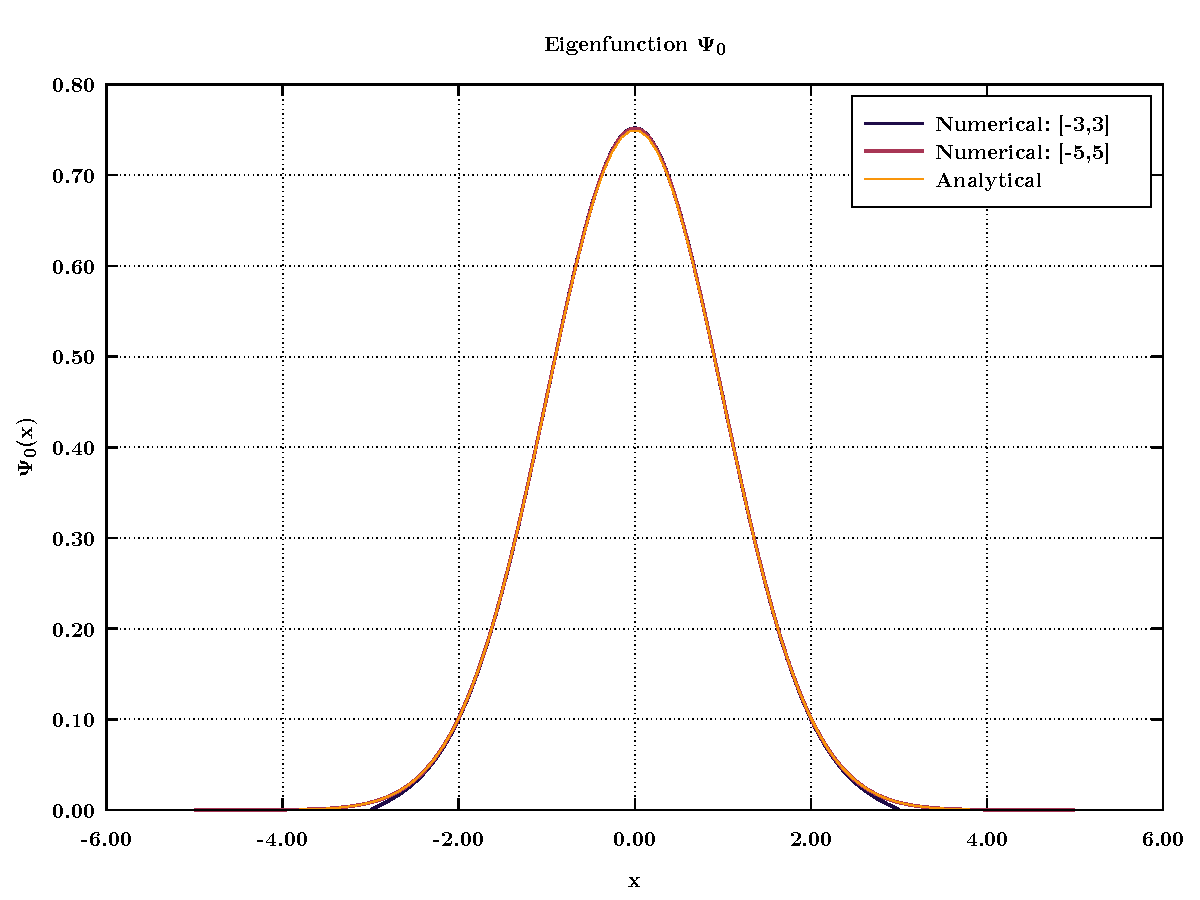
\includegraphics[width=1\textwidth]{image/eig_func_1.pdf}
\end{minipage}
\begin{minipage}[]{0.48\linewidth}
\centering
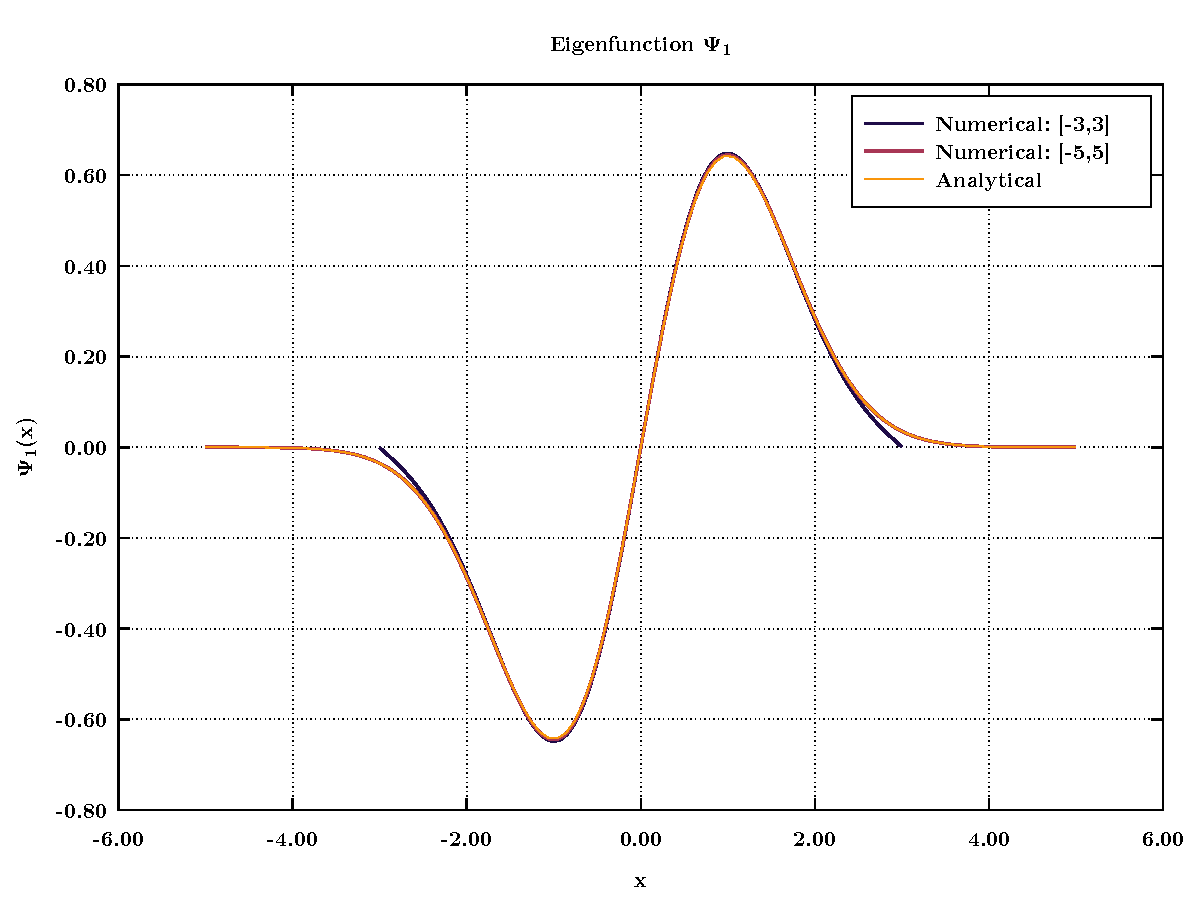
\includegraphics[width=1\textwidth]{image/eig_func_2.pdf}
\end{minipage} \\
\begin{minipage}[c]{0.48\linewidth}
\centering
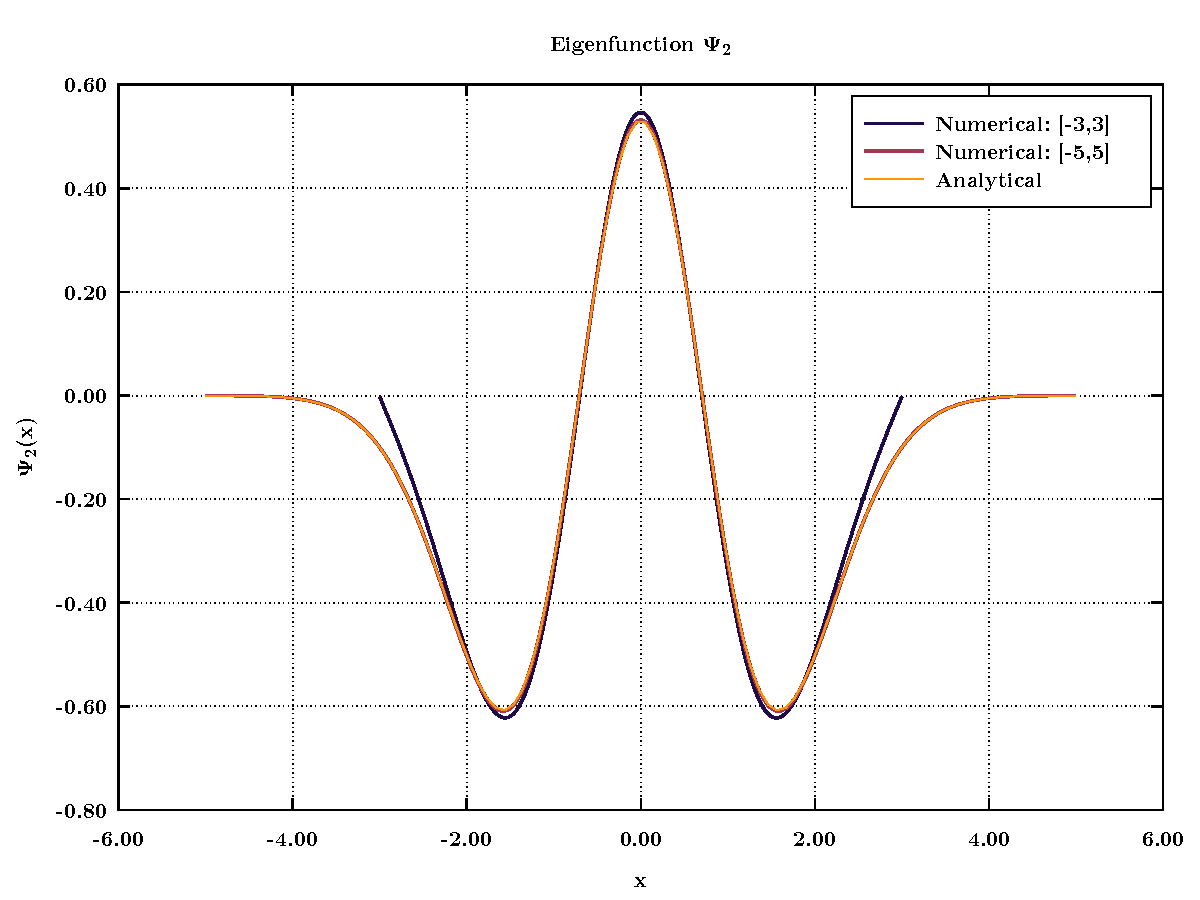
\includegraphics[width=1\textwidth]{image/eig_func_3.pdf}
\end{minipage}
\begin{minipage}[]{0.48\linewidth}
\centering
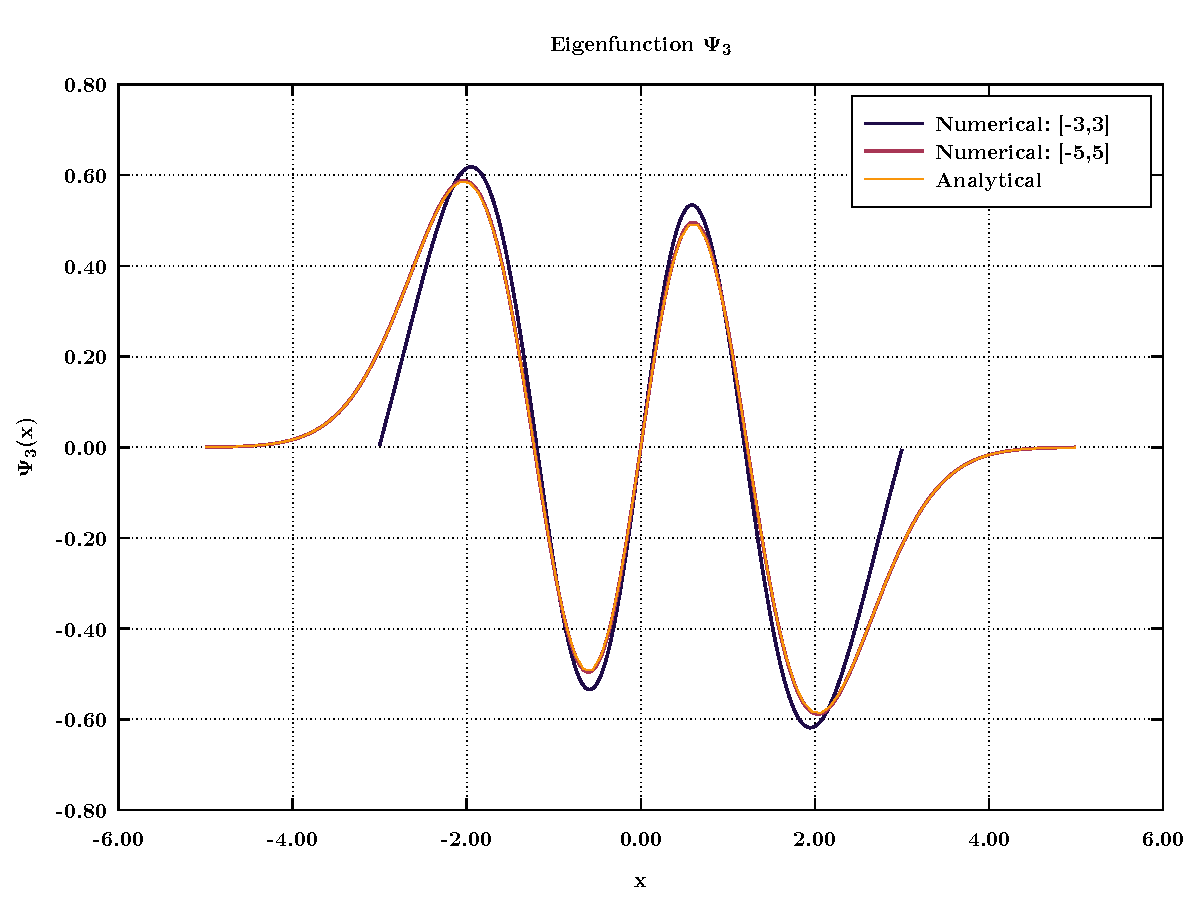
\includegraphics[width=1\textwidth]{image/eig_func_4.pdf}
\end{minipage}
\caption{\label{fig:result_eigenfunc} Plot of first four numerical eigenfunctions for a quantum harmonic oscillator with a space interval of \( [-3,3] \) and \( [-5,5] \). The numerical functions are compared with the analytical ones.}
\end{figure}

\begin{figure}[h!]
\centering
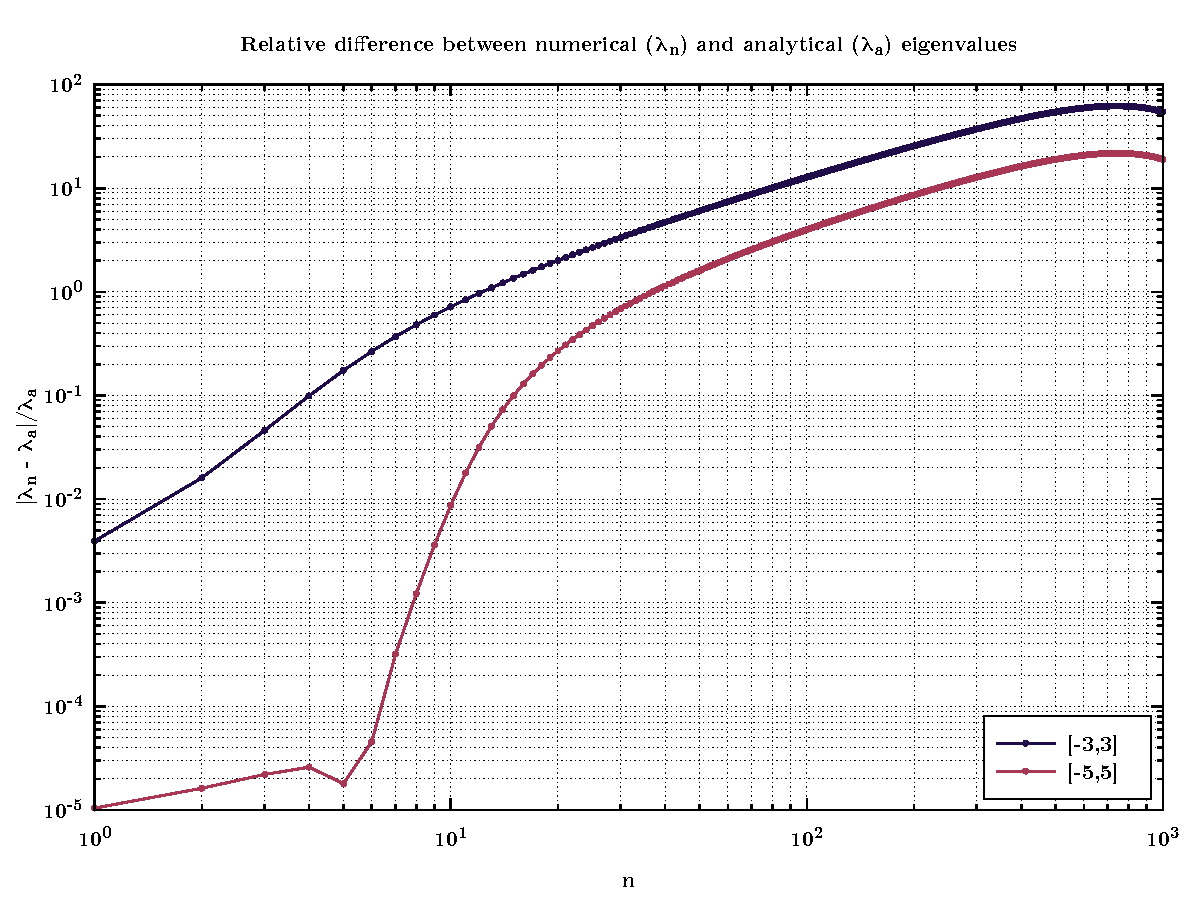
\includegraphics[width=0.5\textwidth]{image/diff_eig_val.pdf}
\caption{\label{fig:result_eigenval} Plot of relative difference between numerical and analytical eigenvalues for \( [-3,3] \) and \( [-5,5] \) space intervals.}
\end{figure}









\section{Self-evaluation}
Let us rate our program in terms of the priorities for good scientific software development:
\begin{itemize}
\item \textbf{correctness}: if we consider lower degree eigenfunctions, for a proper choice of space range, the obtained results perfectly match the theoretical one. Hence, the code is correct but still limited by the discretization and range we used;

\item \textbf{stability}: the code is numerically stable since it returns the same results by running it several times and with several paramters;

\item \textbf{accurate discretization}: accurancy can be further improved by choosing a lower discretization step;

\item \textbf{flexibility}: for the sake of simplicity, we impose \( \omega =1, \hbar =1, m=1 \) in the main program; however, the program can be easily adapated for other values of the parameter for the quantum harmonic oscillator system;

\item \textbf{efficiency}: the program is quite efficient and run in few seconds if we choose a slice dimension of \( N=1000 \) or also \( N=2000 \). Indeed, in the main program we exploit the fact that the hamiltonian is  tridiagonal by finding eigenvalues and eigenvector with the specialized Lapack's function for tridiagonal matrices which are faster than generic ones.
\end{itemize}









\end{document}
